\documentclass[11pt,a4paper,oneside]{article}
\usepackage{graphicx}
\usepackage[utf8]{inputenc}
\usepackage[export]{adjustbox}

%if you don't like the style, comment from here
\setlength{\textwidth}{16cm}
\setlength{\marginparwidth}{1.5cm}
\setlength{\parindent}{0cm}

\setlength{\parskip}{0.15cm}
\setlength{\textheight}{22cm}
\setlength{\oddsidemargin}{0cm}
\setlength{\evensidemargin}{\oddsidemargin}
\setlength{\topmargin}{0cm}
\setlength{\headheight}{0cm}
\setlength{\headsep}{0cm}

\renewcommand{\familydefault}{\sfdefault}
%until here to see the old style

\begin{document}
\graphicspath{ {images/} }
\title{Designing an Index for ZooDB}
\author{Jonas Nick \& Bogdan Vancea}
%\date{December 2004}
\maketitle
\tableofcontents

\section{Introduction}
ZooDB is an open source object database written in Java. It is based on the JDO standard, which is a specification of Java object persistence.
At this point it lacks some advanced features like concurrency and schema evolution but it has been applied successfully in some university projects. Its selling point is speed on the pole position benchmark.
\subsection{Database Index}
 The following definition captures what we want to understand as a database index.
 Here is an example where a user of the database creates an index. He has a class Person and wants to retrieve instances of the class rapidly by name.
 This is called an Attribute Index, which maps values (here names) to Object-IDs
 ZooDB uses Indexes on several other places, it has for example an ObjectID index to map OIDs to positions on the disk and an Extension Index to map a Diskposition to the following Diskposition if an Object spans several disk pages. 

\subsection{B+-Tree}
 What can be the underlying data structure of an Index? We said that the Index should allow for ordered iteration which makes an ordered data structure such as a search tree ideal. Further, the index is going to be stored in a file on the hard drive, which is why indexes are implemented as B+-Trees
 This is an example of a B+-Tree, which has an inner node that contains keys and pointer to children and leaf nodes that contain keys and values, which are depicted here as dots.
 The most important property of a B+-Tree is that a node fills exactly one disk page, which is why the leafs in the example have space here for other keys.
 This means that a node has a maximum number of entries and in order to use as few disk pages as possible the nodes should be as full as possible, meaning that there is a minimum number of entries that are allowed in a node. This is normally a half of the maximum number of keys.

 Here is an example for inserting the entry with key 8 and some value. We see that 8 is smaller than 13, so we have to insert the entry into this leaf. This node would not fit on a disk page anymore so we have to split it in half.
 And since there are now more children of this parent node, there has to be another key in this node too. So 5 is the key that is copied to the upper level.
 Now the parent page overflows so the node is split in half and one key goes to the upper level. 
 Leading to this tree, which is balanced and the requirements of minimum and maximum entries are still fulfilled (except in the root).

 As we have seen re-balancing on insert takes place by using splits. When deleting an entry and the node becomes underfull, the node is merged with a sibling node. If a merge is not possible, some entries are redistributed from a sibling to the underflowing node.
 All operations have logarithmic time complexity.


\section{Goals \& Challenges}
 We had several goals in this project.
 ZooDB already had an Index, our reimplementation should be significantly faster. The index implementation has a substantial impact on the performance of the whole database
 There should be two types of indices, one key unique and one key-value unique. 
   The difference is that in a key unique index the first entry will be overwritten, in a key-value unique index, both entries can exist. 
 The index should support range query iterators
 Also, the index should support caching using a buffer manager. Basically the buffer manager is responsible for fetching pages from disk and provide them to the B+-tree.
 And the Index should use prefix-sharing, a technique I am going to explain next.

\subsection{Prefix sharing}
 Imagine this box represents a node which has some keys. 
 The bit-prefix of all keys is the same, so we can store only the deviations from the prefix.
 You can easily see that we have to store less bits now, meaning that we can pack more keys on a page.
 Prefix sharing introduces a lot of changes to the logic of the BTree. With prefix sharing every node can have a variable number of entries, depending on the actual keys. Previously, the maximum number of entries was the same for all nodes. This means that prefix sharing also affects all re-balancing operations.

\subsection{Challenges}

 The runtime of the index is dominated by disk access, therefore having fewer pages meaning fewer nodes is preferred.
 And since modified nodes have to written to disk, you want to rarely modify nodes.
 New features are costly, prefix-sharing encoding takes time and caching adds another layer of indirection.
 Textbook algorithms need to be adapted because they are not optimized for our practical scenario in various ways (sibling pointer, different order).
 and they do not cover prefix sharing nor dealing with duplicates. The operations for key-value unique trees are in many steps different.
 And we dealt with low level implementations: replacing multiplications/divisions with bit-shifts and reducing polymorphism

\section{Implementation}
\subsection{Buffer Manager} % (fold)
\label{sub:buffer_manager}
Explain how all accesses to nodes are done through the BufferManager.

\subsection{Class Diagram} % (fold)
\label{sub:class_diagram}

For the new implementation of the index we have focused on achieving a balance between good design and code that offers good performance. Figure \ref{fig:class-diagram} show the class diagram for ZooDB.  
\begin{figure}[h]
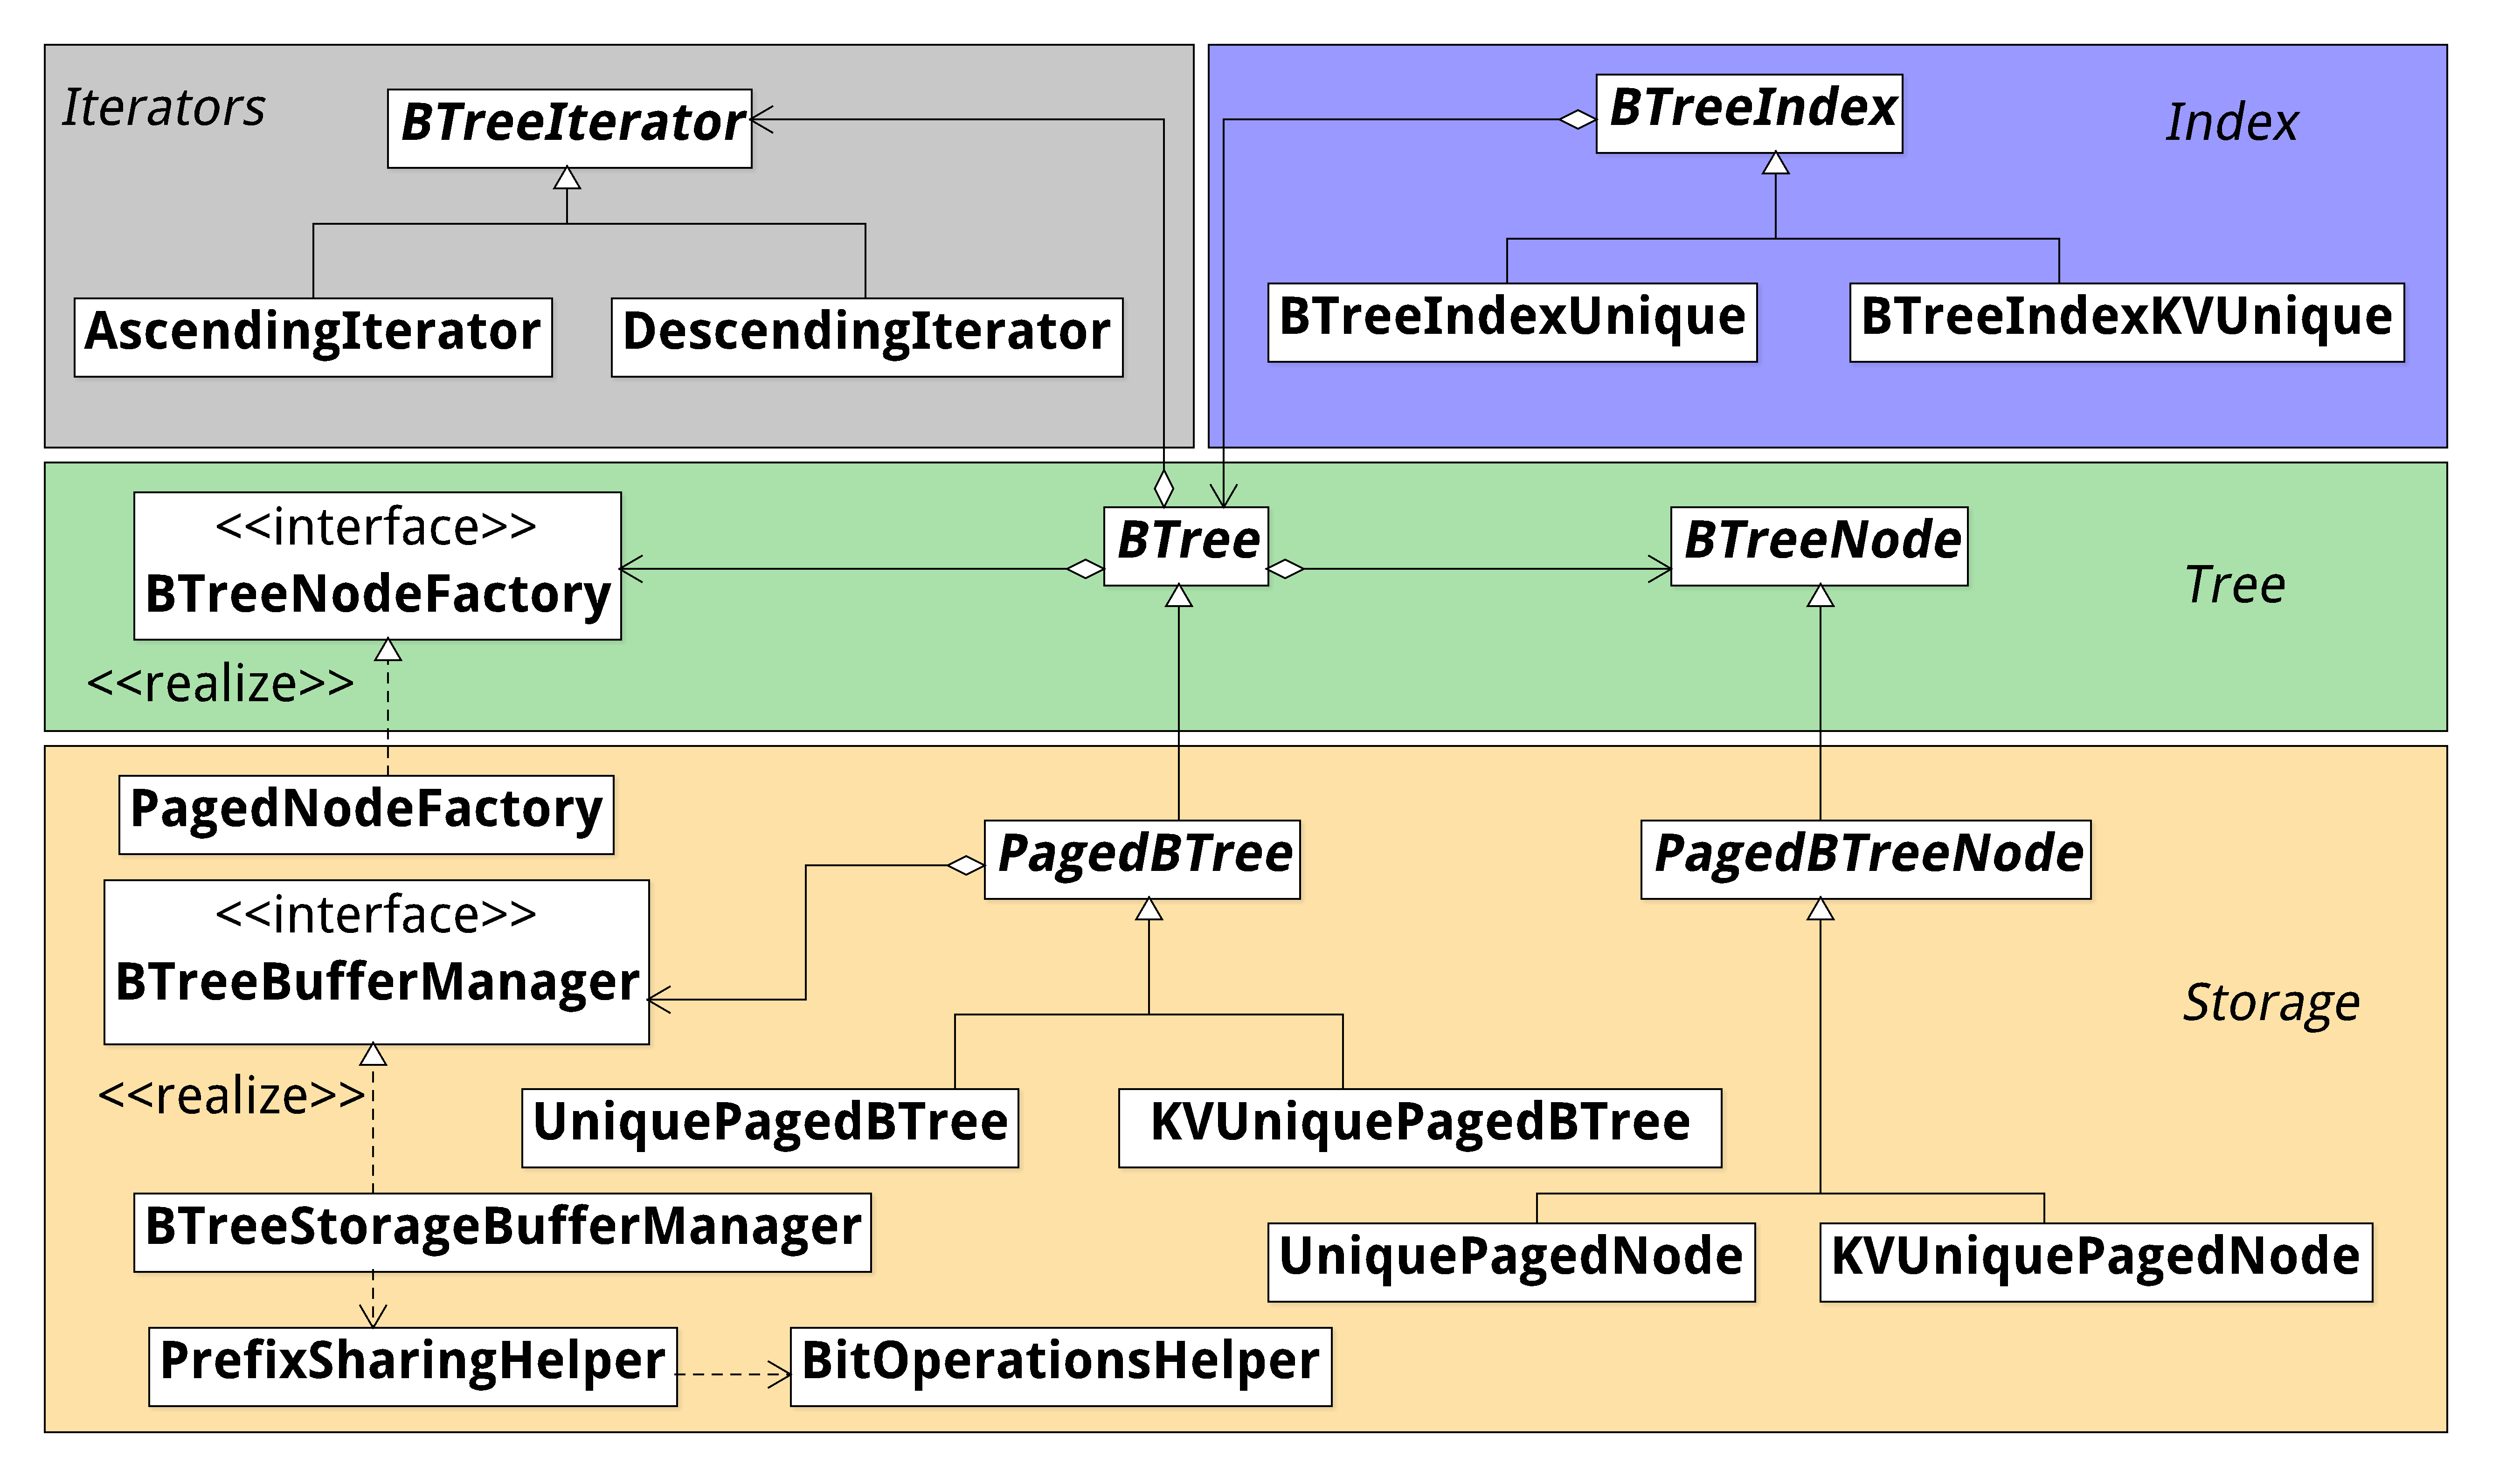
\includegraphics[scale=0.089, center]{ZooDBClassDiagram} 
\caption{The class diagram for the new index implementation}
\label{fig:class-diagram}
\end{figure}

% subsection subsection_name (end)
The \textbf{BTree} class implements all the logic for the B+ tree operations, including the re-balancing operations. The operations implemented operate on instances of the \textbf{BTreeNode} class. The \textbf{BTreeNode} abstract class contains the logic for a B+ tree node. To reduce the usage of polymorphism, we have opted not to implement different classes for leaf, inner or root nodes. The \textbf{BTreeNode} class has additional boolean fields, \textit{isLeaf} and \textit{isRoot} that are used to describe the position of a node within the tree. This choice reduces the size of the inheritance hierarchy, however in the cases where leaf nodes have to be treated differently than inner nodes we have added additional if statements to separate the behavior. 

The \textbf{BTreeNode} class holds no information about the child nodes of the node. However, this class exposes a number of abstract child access methods, like \textit{getChild()} or \textit{getChildren()}. These methods are implemented by the \textbf{PagedBTreeNode} class. Additionally, the \textbf{BTreeNode} class does not hold any information to differentiate between nodes belonging to unique and non-unique trees. All of the methods of for the \textbf{BTree} and \textbf{BTreeNode} classes which need to have different behaviour for unique and non-unique trees are abstract methods and will be overridden by the \textbf{UniquePagedBTreeNode} and \textbf{NonUniquePagedBTreeNode} classes.

The \textbf{PagedBTreeNode} holds the logic responsible for loading nodes from storage. class extends the \textbf{BTreeNode} and contains a reference to the BufferManager associated with the tree. Each instance of \textbf{PagedBTreeNode} contains a \textit{pageId}, which is given assigned by the \textbf{BufferManager} upon storage. The \textbf{PagedBTree} node contains information about the children of a node. We have opted to store the an array consisting of the page ids of the child nodes, instead of an array of hard references to the PagedBTreeNodes. Instead we store an array of weak references to the \textbf{PagedBTreeNode} objects. When a new node is loaded from disk, the child array is populated with the page ids of its child nodes while the array of weak references to the children is initialized to an array of null references. The first access to a child node will retrieve the \textbf{PagedBTreeNode} instance from the buffer manager and populate the weak references corresponding to its page id. Subsequent accesses to the child will use the weak reference, provided the child objects is not reclaimed by the garbage collector. If any of the children nodes are reclaimed by the garbage collector, they will be retrieved from storage on the next access and the weak reference will be repopulated.

The \textbf{UniquePagedBTreeNode} and \textbf{NonUniquePagedBTreeNode} classes extend the \textbf{PagedBTreeNode} class and contain data and behaviour specific to nodes belonging to unique and non-unique trees. For example, in case the non-unique nodes, inner nodes cotains the both a key array and a value array. This leads to different behaviour for unique and non-unique nodes during operations like peforming binary searches, shifting node entries to the left or right or copying node entries from one node to the other. This different behaviour is implemented in the aforementioned classes: \textbf{UniquePagedBTreeNode} and \textbf{NonUniquePagedBTreeNode}. 

The tree iterators are implemented by the \textbf{AscendingBTreeLeafEntryIterator} and \textbf{DescendingBTreeLeafEntryIterator} classes. The shared behaviour for these classes is implemented in the abstract class \textbf{BTreeLeafEntryIterator}. Because we have opted not to store information about the parent nodes, neither in the form of page ids or references, the iteration process requires the use of a stack to store the current position in the tree. The iterators do not support \textbf{Copy on Write} and are invalidated when the B+ tree is modified. 

The indexes are implemented in the \textbf{UniqueBTreeIndex} and \textbf{NonUniqueBTreeIndex} classes. As the index interface offers both methods to modify the B+ tree and to create iterators, we have opted to separate the tree logic in \textbf{BTree} and the iterator in \textbf{BTreeLeafEntryIterator}. This means that index objects delete all B+ tree operations to a reference of a \textbf{BTree} and create instances of \textbf{BTreeLeafEntryIterator} as needed.

The prefix sharing logic has been implemented in the \textbf{PrefixSharingHelper} class. Operations like computing the prefix, encoding/decoding the key array using prefix sharing and the re-balancing computations are available as static methods. We have choses to keep all this logic static to avoid creating extra computational objects that would have to be passed to \textbf{BTreeNode} objects upon creation.
% subsection class_diagram (end)

\subsection{B+ Tree Operations} % (fold)
\label{sub:b_tree_operations}
One important implementation choice we have made is to store the key array un-encoded in memory and to perform the prefix sharing encoding only when nodes are written to disk. While this approach increase the size of the node pages when loaded in memory, the advantage of this choice is that the costly key array encoding is only performed once, even if the node is modified multiple times before it is written to disk. 

Another advantage of having the key array unencoded in memory is that the search operations is similar to the search operation run on a traditional B+ tree. 

For the insert operation, if the new key has been inserted in the first or the last position of the key array, the prefix for the node has to be recomputed. The overflow is handled as follows:
\begin{enumerate}
	\item The algorithm first attempts to redistribute some keys from the current node to its left sibling. We do this to delay the moment when a new node is created. The exact redistribution process is described in the next section.
	\item If that is not possible, the current node is split into 2 nodes of equal size. One important different appears in how the new tree handles keys moving from one node to the other. In a traditional B+ tree, the max number of keys on a node is fixed, which makes it very to perform operations like splitting a node into 2 nodes of equal sizes. In case of prefix sharing, the first half of the keys could have a very different prefix size compared to the second half, which would lead to having 2 nodes with very different sizes. To avoid this, we perform a binary search to compute the optimal number of keys to move to the new node.
\end{enumerate}
	
In the case of the delete operation, the removal of an entry from the key array can cause the prefix to change. If the node from which the deletion has been performed is now underfull, a re-balancing procedure begin. The steps for the re-balancing are the following:
\begin{enumerate}
	\item In the first step, the algorithm first checks if the current node can be merged with \textbf{either} its left or its right neighbour. 
	\item If the merge at the previous step is not possible, the next step is to check wether the keys from the current node can be split between its left sibling \textbf{and} its right sibling. While this approach would involve in marking both the left and righ siblings as dirty, the current node can then be removed.
	\item If the the previous operation was not possible, some keys are redistribute from either the left or the right sibling. As a note, the success of the rebalancing operations is not guaranteed and the current node could remain underfull after the re-balance operation. However, we observed that this behaviour does not happen very often and does not have a significant impact on the tree size.
\end{enumerate}

% subsection b_tree_operations (end)

\subsection{Prefix Sharing Implementation} % (fold)
\label{sub:prefix_sharing_rebalancing}
When storing a node, the key array of a node is encoded into an array of bytes accoding to the common prefix. The encoding was peformed at the bit-level, meaning that both the binary prefix and the deviations of elements from the prefix are computed as arbitrary number of bits. This means that if the binary prefix has length 9, it can be store in 2 bytes. Moreover, the remaining 7 bits from the second byte can be used to store part of the deviation of the fist array element. Other available alternatives for encoding would have been to compute both the prefix and the deviations as multiples of 8 and ensure that each encoded byte contains only prefix bits or deviation bits. We have chosen the bit-level encoding because it offers the best space reduction.

We have based the prefix sharing algorithms on the following observations about the binary prefix for an array of \textbf{sorted} integer elements.
\begin{itemize}
	\item The binary prefix of the array is equal to the binary prefix shared by the first and last element.
	\item Inserting a new element in the array in an ordered manner will either decrease the prefix of the whole array or leave it unchanged.
	\item Removing an element from the array will either increase the prefix of the whole array or leave it unchanged.
\end{itemize}

Details about split.

Details about merge.

Details about redistribute.

\subsection{Support for different sizes}
We have support for this (ex: PagedPosIndex) , maybe we can provide some additional details.


% subsection prefix_sharing_rebalancing (end)


\end{document}
